\documentclass{article}
\usepackage{graphicx}
\usepackage{amssymb}
\usepackage{amsmath}
\usepackage{hyperref}

\title{Hashing Table Prefixing Implementation Report}
\author{Ziyuan Lin}
\date{2024.3.17}

\begin{document}

\maketitle

\section{Basic Idea of Hash Prefix Caching}
In this small project, I implement the prefixing caching using hash table. With the modern hash function, the collision rate will be extremely small.
Hence any block will be totally determined by its prefix and own tokens. Thus \\ $hash(prefix, own)$ uniquely defines a block. Using this prefix technique, all sequences in the entire life cycle of the engine can share the prefix.
Reducing the time for allocation and computation. When a request finishes, we do not immediately remove the cache. Instead, we fix a pool of prefix cache with maximum size $K$ as a hyperparameter. When a block is freed, the block is added into the
pool. When the pool is full, the cache pool starts to evict the block from the pool. The eviction policy is to remove block first based on the last utilized time, then on the prefix length of the block. The later the block being used implies that the block 
is frequently used, hence last to remove. For the blocks with the same last touch time, remove the block with the longest prefix to prevent from removing the token in the middle. 

\section{Experimental Results}
The experiment shows that adding hashing prefix cache can indeed improve the performance. However, this can only be achieved in some extreme scenario. In this section, I am going to present some results and explain the reasons behind these results.
\subsection{Random Prompt Generator}
I create a random prompt generator. The generator has a pool of frequent sequences. For each loop, it has probability $p$ to select a request from the pool, and $1-p$ probability to generate a random request with length $15$.
I generate 1000 requests to form the prompt.
\\[8pt]
\subsection{Hit rate}
Range $p$ from 0.1 to 1.0. Here is how hit rate changes. In this work, the hit rate is counted only once for the initial prompt. 

\begin{figure}[h]
    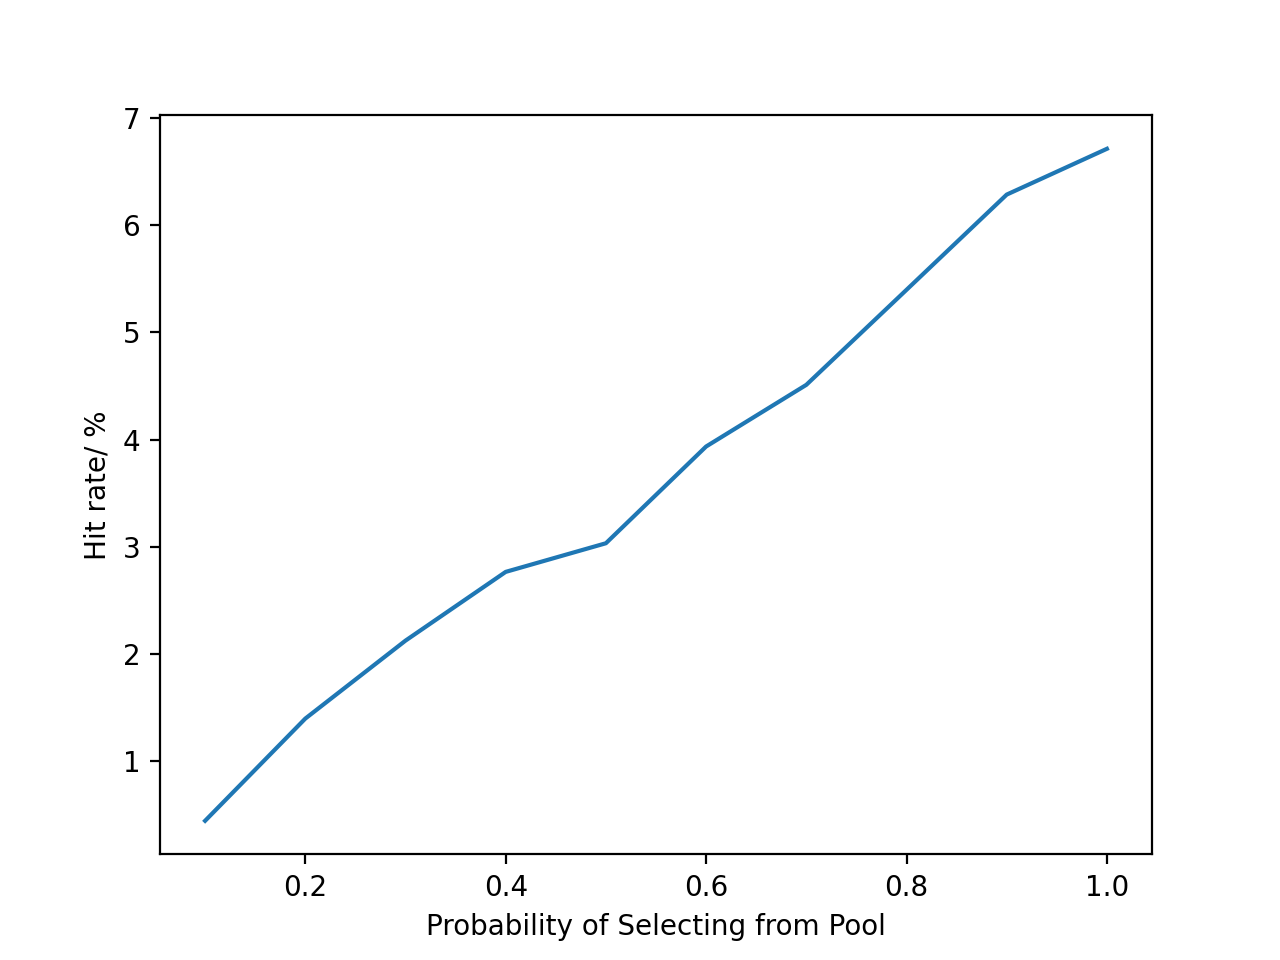
\includegraphics[scale = 0.4]{Hit_rate.png}
    \centering
    \caption{Hit rate vs Sampling probability}
    \label{fig:}
\end{figure}

As we can see, hit rate increases almost linearly with respect to probability of sampling from the pool. I also test the case with only one type request. For instance, the hit rate of sequence
"What is your name?" is $8.14\%$. This totally makes sense since as $p$ increases, matched or closed matched sequences increases. For identical sequences, $8.14\%$ is not that high because the generated sequences are different even
though they have the same prompt tokens.

\subsection{Performance}
I use the items per second as the metric for performance. Figure $2$ shows how the items per second changes with respect to $p$. Note that the average items per second for non-prefixing version is $416.92$.
\begin{figure}[h]
    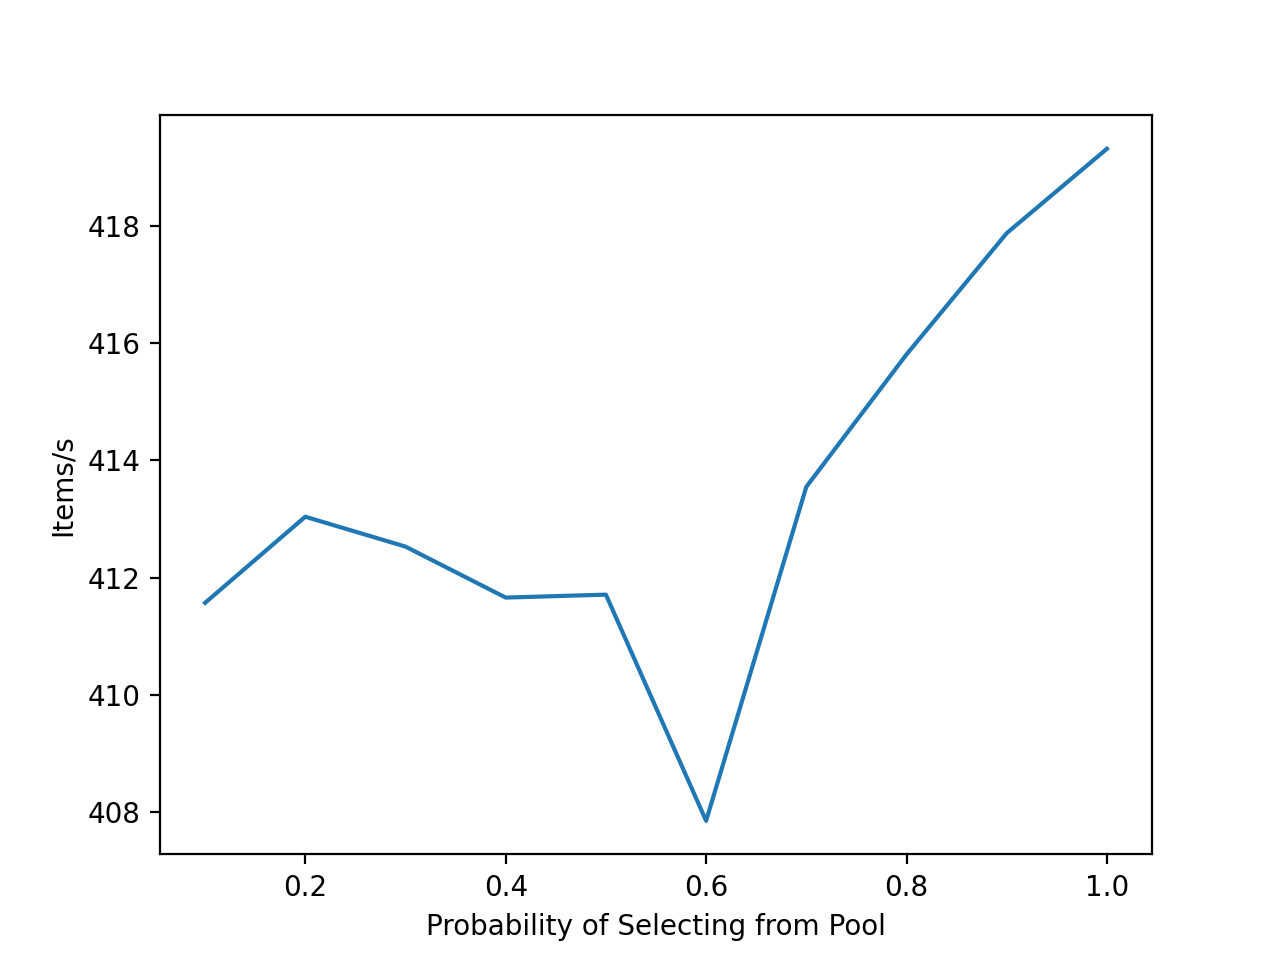
\includegraphics[scale = 0.4]{Performance.png}
    \centering
    \caption{Items per second vs Sampling probability}
    \label{fig:}
\end{figure}

We note that the performance is not quite stable compared to the hit rate. This is due to two factors. On the one hand, the new scheme needs extra work on calculating the hashing value and managing the cache pool.
On the other hand, the randomness causes large difference in requests, hence quite different final sequence length. However, we can see that even with extra work, the performance of the hashing prefix version still outperforms
original no prefixing case for large enough $p$. For the extreme case of identical prompts, the performance is even better. For instance, "What is your name?" achieves 459.22 items/s.

\section{Future Work}
Here I list $3$ potential future work: (1) Change the direct hashing to hierarchical hashing. That is assume that each block is identified by $hash(prev\_hash, own)$. This assumption should holds since even with hierarchy, the hit rate is 
still small. (2) Change the eviction policy. We may change the eviction policy. For example, the first criterion may be based on the frequency touched by gpu. (3) Further experiment. I think current experiment is not enough to understand the whole story.
More prompts can be tried. Also I need to find a better performance criterion.

\end{document}